%!TEX TS-program = xelatex
\documentclass[notes,12pt, aspectratio=169]{beamer}

\usepackage{amsmath,amsfonts,amssymb,amsthm,mathtools}  % пакеты для математики
\usepackage{minted}

\usepackage[english, russian]{babel} % выбор языка для документа
\usepackage[utf8]{inputenc} % задание utf8 кодировки исходного tex файла
\usepackage[X2,T2A]{fontenc}        % кодировка

\usepackage{fontspec}         % пакет для подгрузки шрифтов
\setmainfont{Helvetica}  % задаёт основной шрифт документа

% why do we need \newfontfamily:
% http://tex.stackexchange.com/questions/91507/
\newfontfamily{\cyrillicfonttt}{Helvetica}
\newfontfamily{\cyrillicfont}{Helvetica}
\newfontfamily{\cyrillicfontsf}{Helvetica}

\usepackage{unicode-math}     % пакет для установки математического шрифта
% \setmathfont{Neo Euler} % шрифт для математики

\usepackage{polyglossia}      % Пакет, который позволяет подгружать русские буквы
\setdefaultlanguage{russian}  % Основной язык документа
\setotherlanguage{english}    % Второстепенный язык документа

% Шрифт для кода
\setmonofont[Scale=0.85]{Monaco}
\usepackage{verbments}

\usepackage{pgfpages}
% These slides also contain speaker notes. You can print just the slides,
% just the notes, or both, depending on the setting below. Comment out the want
% you want.
%\setbeameroption{hide notes} % Only slide
%\setbeameroption{show only notes} % Only notes
%\setbeameroption{show notes on second screen=right} % Both

\usepackage{array}

\usepackage{tikz}
\usepackage{verbatim}
\setbeamertemplate{note page}{\pagecolor{yellow!5}\insertnote}
\usetikzlibrary{positioning}
\usetikzlibrary{snakes}
\usetikzlibrary{calc}
\usetikzlibrary{arrows}
\usetikzlibrary{decorations.markings}
\usetikzlibrary{shapes.misc}
\usetikzlibrary{matrix,shapes,arrows,fit,tikzmark}

\usepackage{hyperref}
\usepackage{lipsum}
\usepackage{multimedia}
\usepackage{multirow}
\usepackage{dcolumn}
\usepackage{bbm}
\newcolumntype{d}[0]{D{.}{.}{5}}

\usepackage{changepage}
\usepackage{appendixnumberbeamer}
\newcommand{\beginbackup}{
   \newcounter{framenumbervorappendix}
   \setcounter{framenumbervorappendix}{\value{framenumber}}
   \setbeamertemplate{footline}
   {
     \leavevmode%
     \hline
     box{%
       \begin{beamercolorbox}[wd=\paperwidth,ht=2.25ex,dp=1ex,right]{footlinecolor}%
%         \insertframenumber  \hspace*{2ex} 
       \end{beamercolorbox}}%
     \vskip0pt%
   }
 }
\newcommand{\backupend}{
   \addtocounter{framenumbervorappendix}{-\value{framenumber}}
   \addtocounter{framenumber}{\value{framenumbervorappendix}} 
}

% для имитации питоновского синтаксиса 
\newcommand{\pgr}[1]{{\color{green} \textbf{#1}}}


%%%%%%%%%% Работа с картинками %%%%%%%%%
\usepackage{graphicx}                  % Для вставки рисунков
\usepackage{graphics}
\graphicspath{{images/}}    % можно указать папки с картинками
\usepackage{wrapfig}                   % Обтекание рисунков и таблиц текстом

\usepackage[space]{grffile}
\usepackage{booktabs}

% These are my colors -- there are many like them, but these ones are mine.
\definecolor{blue}{RGB}{0,114,178}
\definecolor{red}{RGB}{213,94,0}
\definecolor{yellow}{RGB}{240,228,66}
\definecolor{green}{RGB}{0,128, 0}

\hypersetup{
  colorlinks=false,
  linkbordercolor = {white},
  linkcolor = {blue}
}


%% I use a beige off white for my background
\definecolor{MyBackground}{RGB}{255,253,218}

%% Uncomment this if you want to change the background color to something else
%\setbeamercolor{background canvas}{bg=MyBackground}

%% Change the bg color to adjust your transition slide background color!
\newenvironment{transitionframe}{
  \setbeamercolor{background canvas}{bg=yellow}
  \begin{frame}}{
    \end{frame}
}

\setbeamercolor{frametitle}{fg=blue}
\setbeamercolor{title}{fg=black}
\setbeamertemplate{footline}[frame number]
\setbeamertemplate{navigation symbols}{} 
\setbeamertemplate{itemize items}{-}
\setbeamercolor{itemize item}{fg=blue}
\setbeamercolor{itemize subitem}{fg=blue}
\setbeamercolor{enumerate item}{fg=blue}
\setbeamercolor{enumerate subitem}{fg=blue}
\setbeamercolor{button}{bg=MyBackground,fg=blue,}


% If you like road maps, rather than having clutter at the top, have a roadmap show up at the end of each section 
% (and after your introduction)
% Uncomment this is if you want the roadmap!
% \AtBeginSection[]
% {
%    \begin{frame}
%        \frametitle{Roadmap of Talk}
%        \tableofcontents[currentsection]
%    \end{frame}
% }
\setbeamercolor{section in toc}{fg=blue}
\setbeamercolor{subsection in toc}{fg=red}
\setbeamersize{text margin left=1em,text margin right=1em} 

% списки, которые растягиваются на всю величину слайда 
\newenvironment{wideitemize}{\itemize\addtolength{\itemsep}{10pt}}{\enditemize}



\title[]{\textcolor{blue}{Глубокое обучение и вообще}}
\author{Ульянкин Филипп, Соловей Влад}
\date{\today}


\begin{document}

%%% TIKZ STUFF
\tikzset{   
        every picture/.style={remember picture,baseline},
        every node/.style={anchor=base,align=center,outer sep=1.5pt},
        every path/.style={thick},
        }
\newcommand\marktopleft[1]{%
    \tikz[overlay,remember picture] 
        \node (marker-#1-a) at (-.3em,.3em) {};%
}
\newcommand\markbottomright[2]{%
    \tikz[overlay,remember picture] 
        \node (marker-#1-b) at (0em,0em) {};%
}
\tikzstyle{every picture}+=[remember picture] 
\tikzstyle{mybox} =[draw=black, very thick, rectangle, inner sep=10pt, inner ysep=20pt]
\tikzstyle{fancytitle} =[draw=black,fill=red, text=white]
%%%% END TIKZ STUFF

% Title Slide
\begin{frame}
\maketitle
\centering Введение в RL 
\end{frame}


% слайды про постановку задачи reinfircment learning 
\begin{frame}{Reinforcement Learning}
\begin{center}
	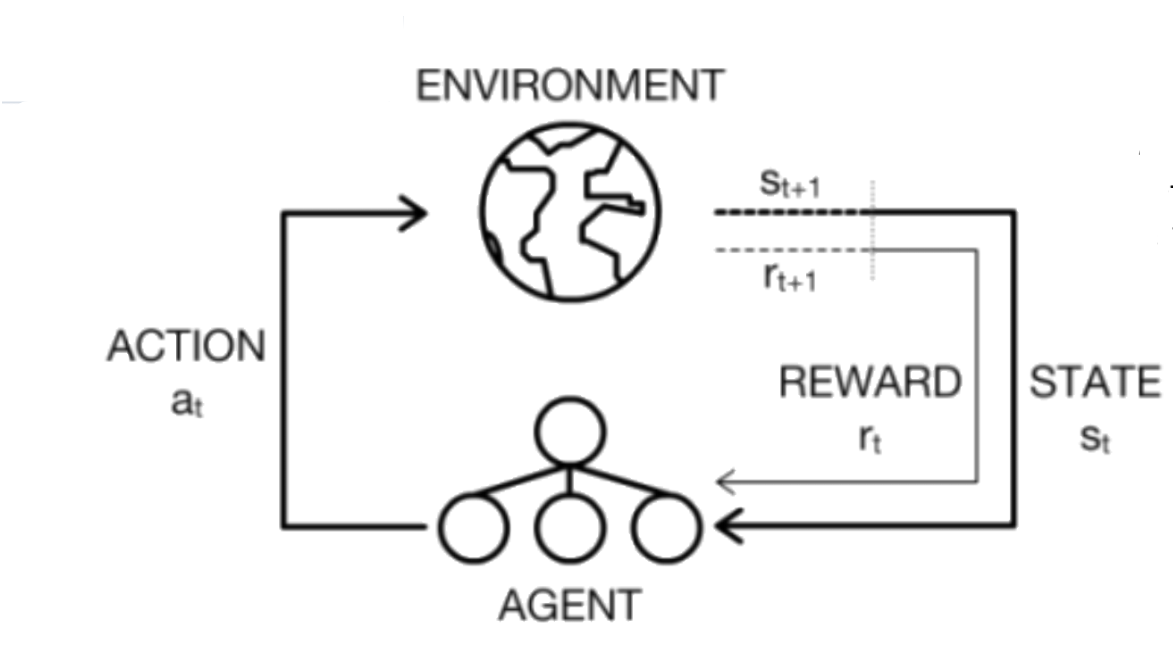
\includegraphics[width=.6\linewidth]{rl_1.png}
\end{center}
\end{frame}


\begin{frame}{Reinforcement Learning}
\begin{center}
	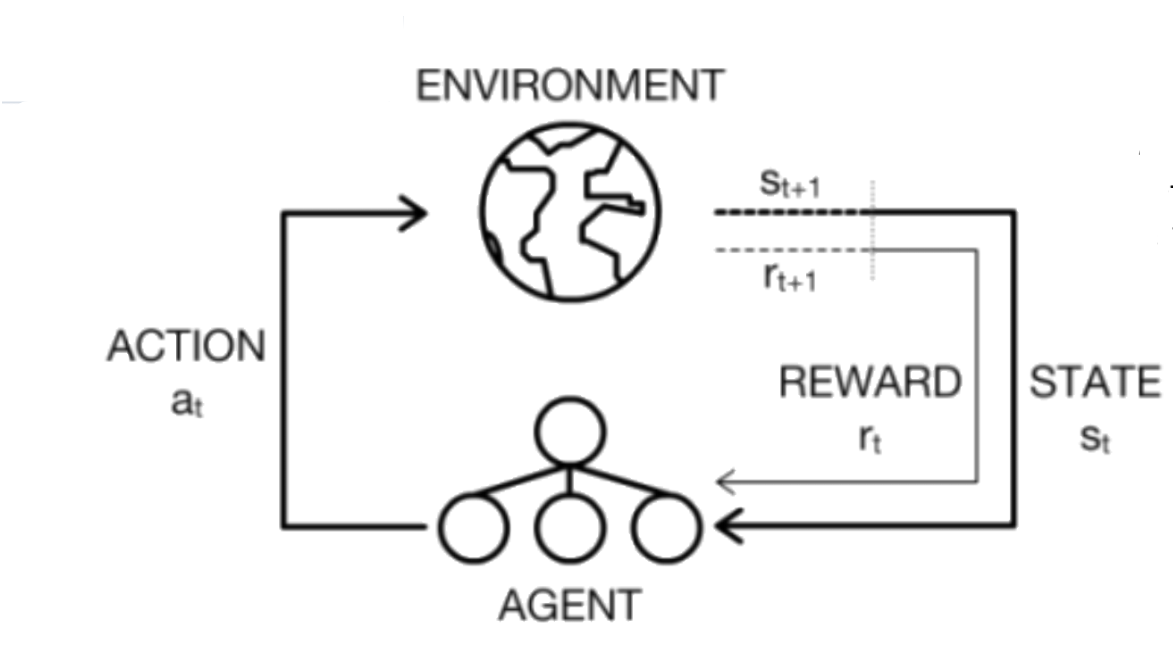
\includegraphics[width=.4\linewidth]{rl_1.png}
\end{center}
\begin{itemize}
	\item  $s_t$ — состояние среды (state);
	\item  $a_t$ — действия агента (action);
	\item  $r_t$ — награда (reward) за действие;
\end{itemize}
\end{frame}


\begin{frame}{Reinforcement Learning}
\begin{center}
	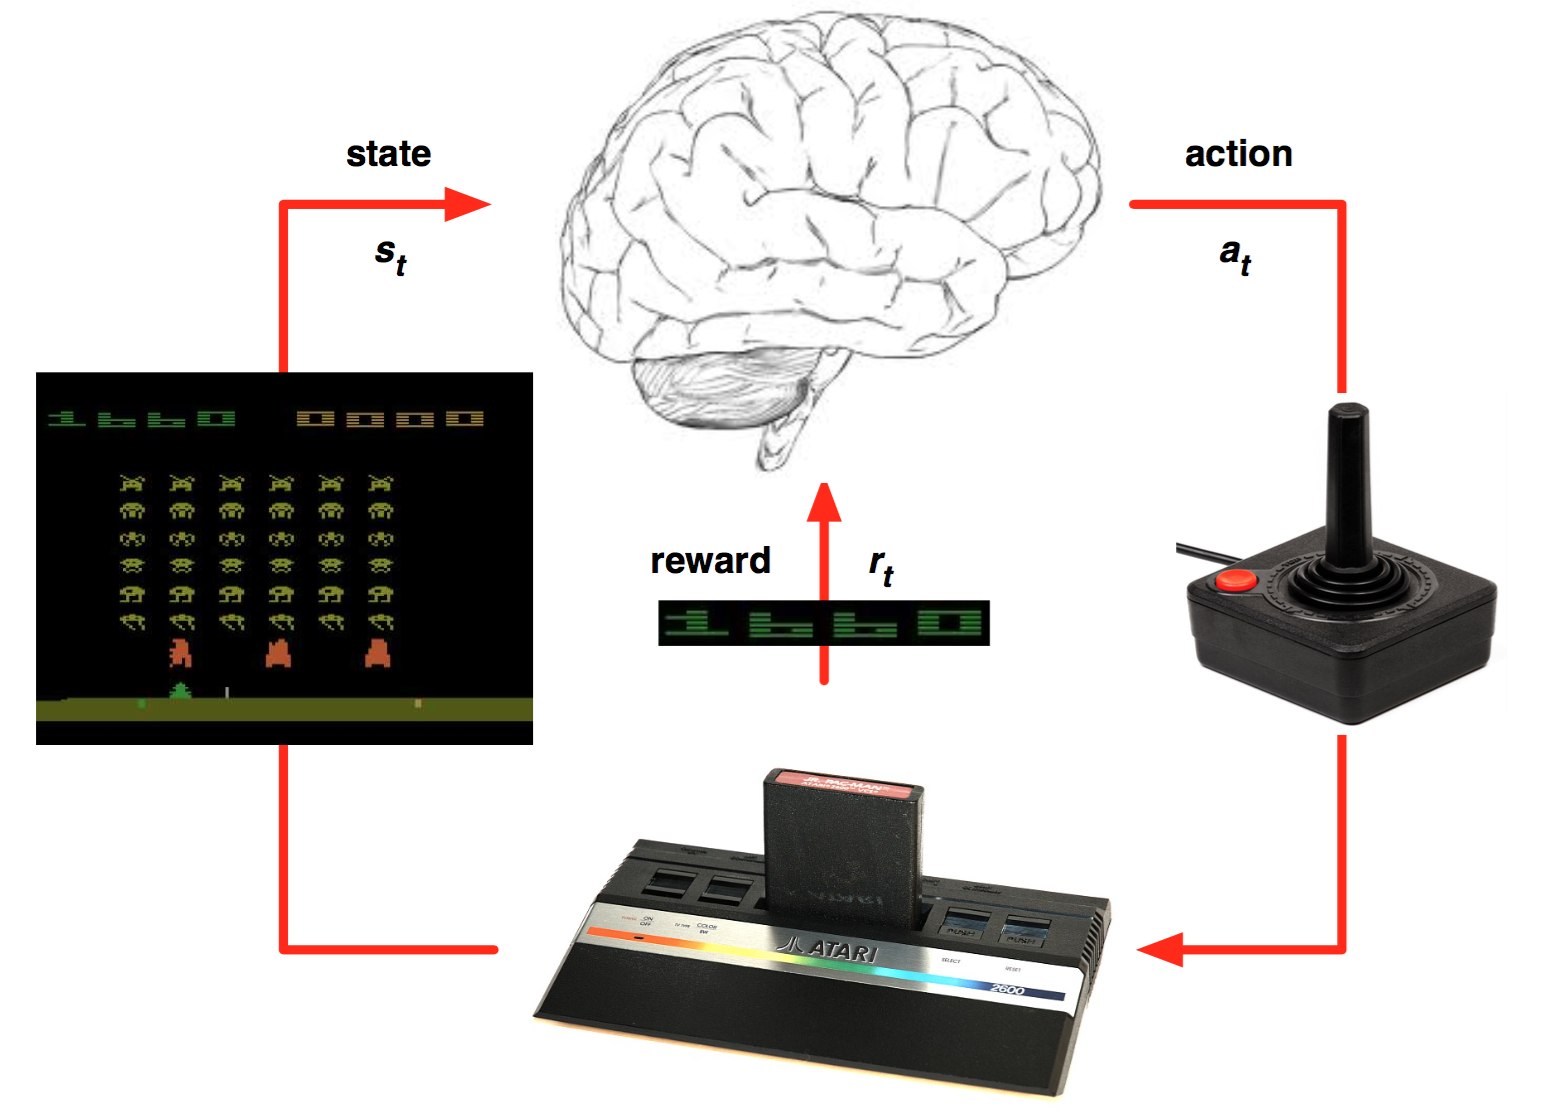
\includegraphics[width=.7\linewidth]{rl_altari.png}
\end{center}
\end{frame}


\begin{frame}{Reinforcement Learning}
\begin{center}
	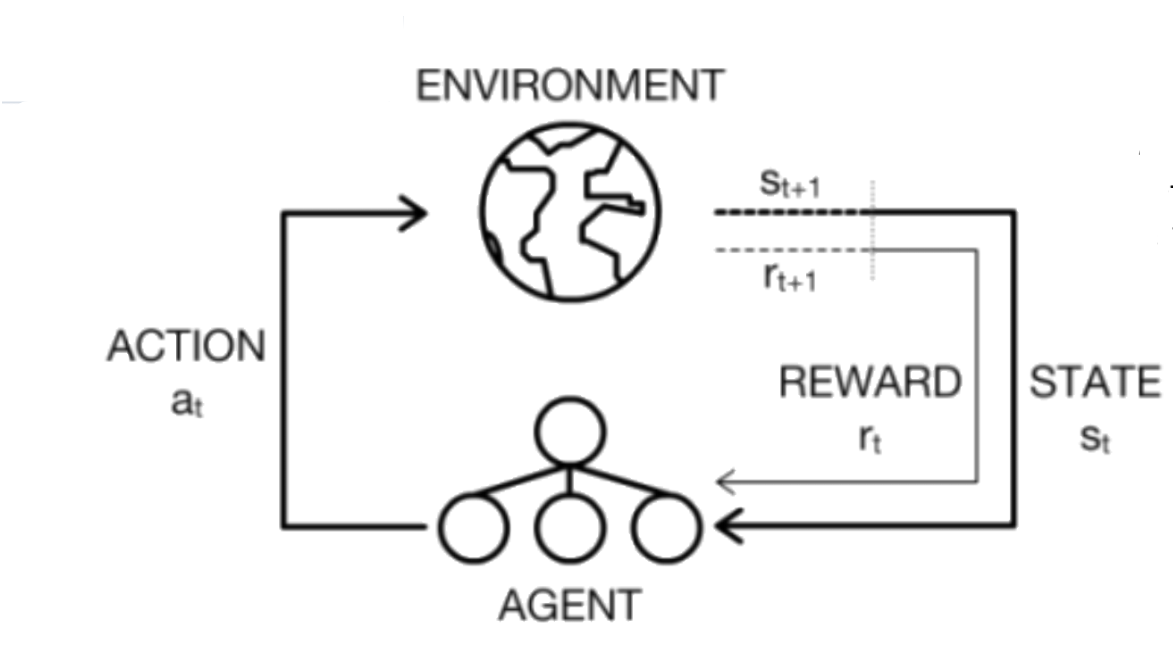
\includegraphics[width=.4\linewidth]{rl_1.png}
\end{center}
\begin{itemize}
	\item  \alert{$v(s)$ — value function,} по state выдаёт оценку всех будущих reward;
	\item  \alert{$p(a \mid s)$ — policy function,} выводит вероятность действия в конкретном состоянии так, чтобы вероятность действия, максимизирующего reward была наибольшей 
	\item  \alert{$Q(s,a)$ — Q-function,} сообщает reward для действия $a$ в состоянии $s$.
\end{itemize}
\end{frame}


\begin{frame}{Reinforcement Learning}
\begin{wideitemize}
\item \alert{Идея:} мы пытаемся выразить действия агента с помощью различных функций. Если мы пытаемся каждую функцию представить в виде нейросетки, мы входим в зону deep reinforcment learning. 

\item В зависимости от того, какую функцию мы оптимизируем, получаем разные алгоритмы 

\item В примере ниже мы будем максимизировать policy function (policy gradient algorithm), после будем заниматься оптимизацией Q-функции (Q-learning)
\end{wideitemize}
\end{frame}


\begin{frame}{Пример: игра в Pong}
\begin{center}
	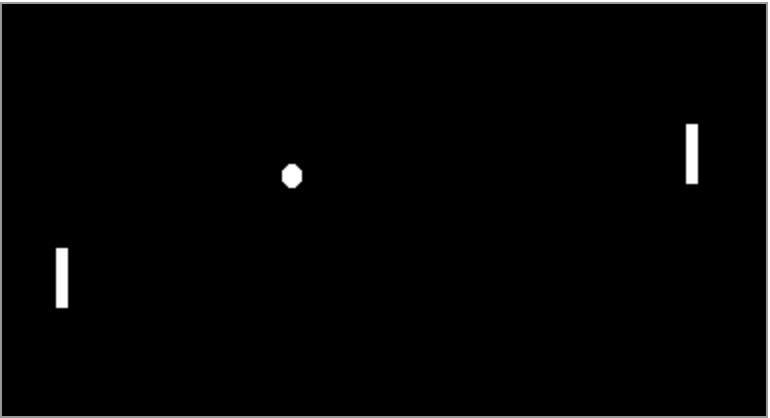
\includegraphics[width=.8\linewidth]{pong.png}
\end{center}
\vfill
{\color{blue}  \url{http://karpathy.github.io/2016/05/31/rl/}}
\end{frame}


\begin{frame}{Пример: игра в Pong}
\begin{center}
	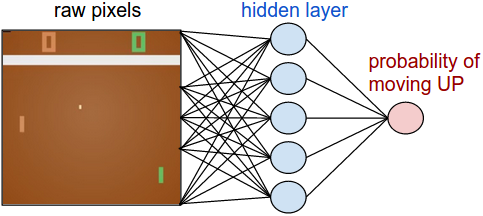
\includegraphics[width=.6\linewidth]{pong_NN.png}
\end{center}
\vfill
{\color{blue}  \url{http://karpathy.github.io/2016/05/31/rl/}}
\end{frame}


\begin{frame}{Пример: игра в Pong}
\begin{wideitemize}
	\item  Хотим натренировать зелёную палку выигрывать! 
	
	\item  Состояние $s_t$ — пиксели экрана
	
	\item Мы хотим обучить нейросеть с одним скрытым слоем, которая по текущему дифу из пикселей предсказывать вероятность движения вверх или вниз 
	
	\item Сеть сама пытается разобраться как правильно играть в эту игру на основе разницы между текущим и предыдущим кадром 
\end{wideitemize}
\end{frame}


\begin{frame}{Пример: игра в Pong}
\begin{center}
	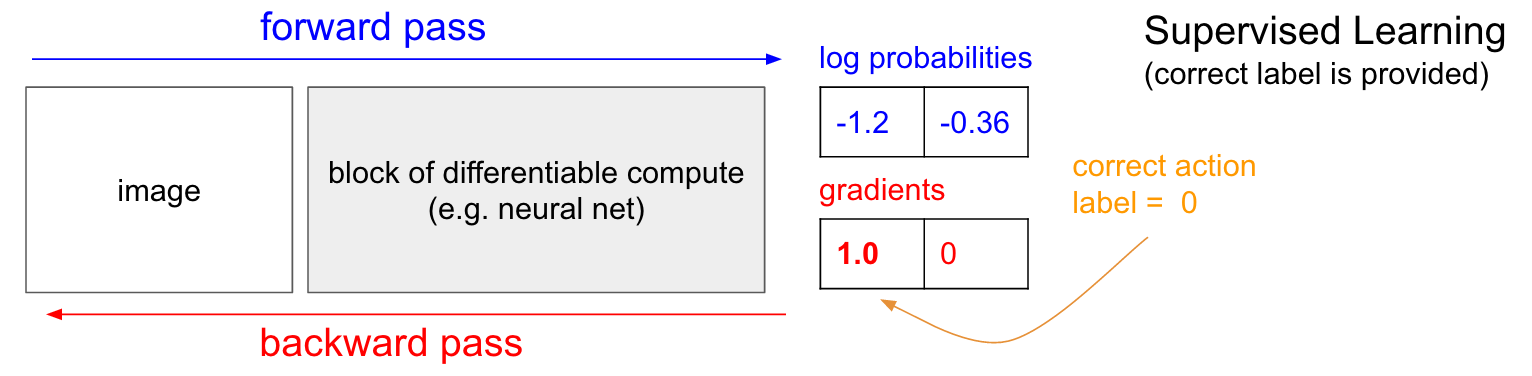
\includegraphics[width=.8\linewidth]{pong_label.png}
\end{center}
\vfill \pause 
\begin{center}
	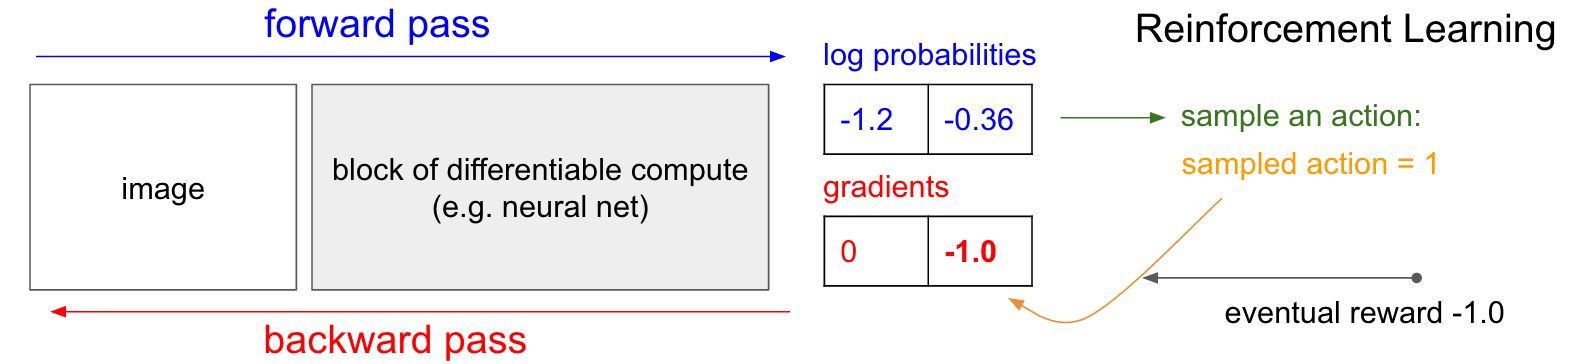
\includegraphics[width=.8\linewidth]{pong_sample.png}
\end{center}
\end{frame}


\begin{frame}{Пример: игра в Pong}
\begin{wideitemize}
	\item   Если бы мы учили обычную сетку, у нас был бы вектор правильных ответов для каждого действия, и мы бы делали backpropagation 
	
	\item  На деле мы знаем результат после многих шагов
	
	\item  Будем передавать вместо таргета то, что произошло на самом деле для последовательности действий 
\end{wideitemize}
\end{frame}


\begin{frame}{Пример: игра в Pong}
\begin{center}
	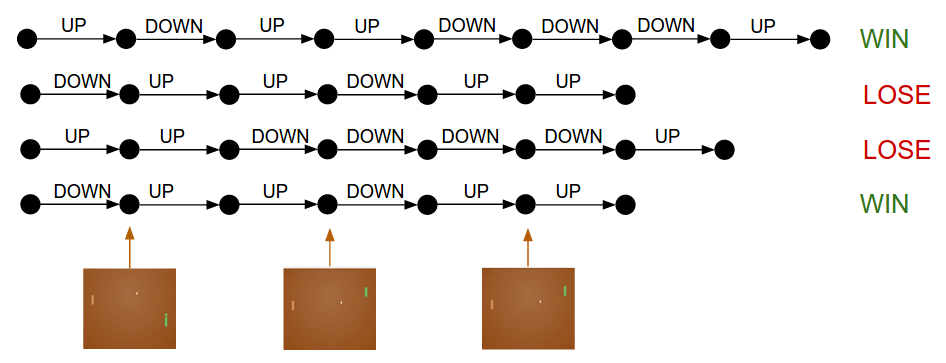
\includegraphics[width=.8\linewidth]{pong_backprop.png}
\end{center}
\end{frame}


\begin{frame}{Почему это работает?}
\begin{wideitemize}
	\item   Пусть $p(a \mid s, \theta)$ — вероятность действия $a$ в состоянии $s$, описываемая параметрами $\theta$, а $f(a)$ — награда от действия $a$
	\item Мы хотим двигать веса $\theta$ так, чтобы средняя награда $E_a [ f(a)]$ увеличивалась
	\item Добиться этого можно с помощью градиентного спуска
\end{wideitemize}
\end{frame}


\begin{frame}{Почему это работает?}
\begin{equation*}
\begin{aligned}
\nabla_{\theta} E_a [f(a)] & = \nabla \sum_a p(a) \cdot f(a) = \\
& = \sum_{a} \nabla_{\theta} p(a) \cdot f(a) = \\
& = \sum_{a} p(a) \cdot \frac{\nabla_{\theta} p(a)}{p(a)} \cdot f(a) = \\
& = \sum_{a} p(a) \cdot \nabla_{\theta} \ln p(a) \cdot f(a) = \\
& = E_a [ f(a) \cdot \nabla_{\theta} \ln p(a) = - logloss \\
\end{aligned}
\end{equation*}
\end{frame}


\begin{frame}{Какой бывает награда}
\begin{center}
	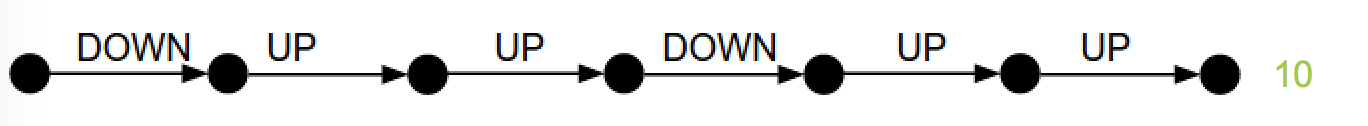
\includegraphics[width=.7\linewidth]{states.png}
\end{center}
\begin{itemize}
	\item В примере выше мы получали награду $r$ за какую-то последовательность действий
	\item Можно определить награду так, что мы её получаем на каждом шаге $r_t$
\end{itemize}
\begin{center}
	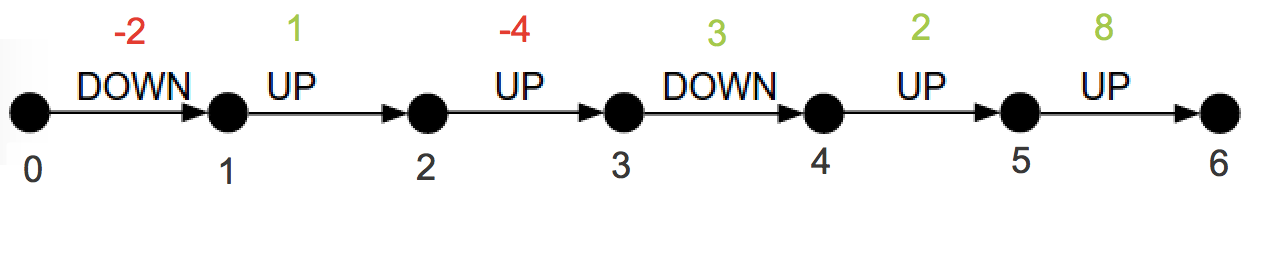
\includegraphics[width=.7\linewidth]{states_1.png}
\end{center}
\end{frame}


\begin{frame}{Какой бывает награда}
\begin{center}
	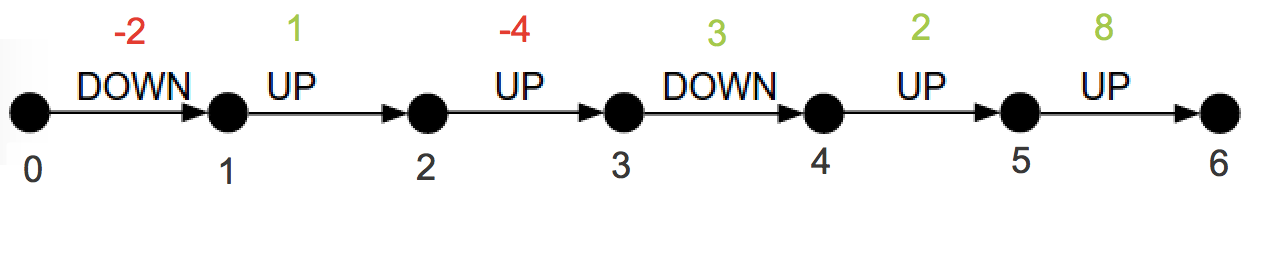
\includegraphics[width=.7\linewidth]{states_1.png}
\end{center}
\begin{equation*}
\begin{aligned}
&R_0 = r_0 + r_1 + r_2 + \ldots + r_{h}  & \qquad  R_1 = r_1 + r_2 + \ldots + r_{h} & \ldots \\
&R_0 = r_0 + \gamma \cdot r_1 + \gamma \cdot r_2 + \ldots +  \gamma^h \cdot r_{h}  & \qquad  R_1 = r_1 + \gamma \cdot r_2 + \ldots + \gamma^{h-1} \cdot r_{h} & \ldots \\
\end{aligned} 
\end{equation*}
\end{frame}


\begin{frame}{Какой бывает награда}
\alert{Фактор дисконтирования $\gamma$} нужен, чтобы очень далёкое будущее влияло на текущее состояние сети не так сильно, как в недалёком. Когда мы просим сеть разобраться с ближайшим будущим, ей легче разобраться в ситуации и обучение стабильнее. 

\vfill 

Иногда агент попадает в очень хорошее состояние и начинает постоянно получать очень большую награду. Из-за этого нейросетке сложно понимать, что $1000$ лучше $999$. Хочется уменьшить масштаб $\Rightarrow$ центрирование и нормирование 
\end{frame}


\begin{frame}
\begin{center}
\alert{\Huge Поздравляю!  \\  \mbox{ }  \\  Вы знаете reinforcment learning \\  \mbox{ }  \\ Остальное — это детали :D } 
\end{center}
\end{frame}

\begin{frame}{Reinforcement Learning - это просто!}
\begin{center}
	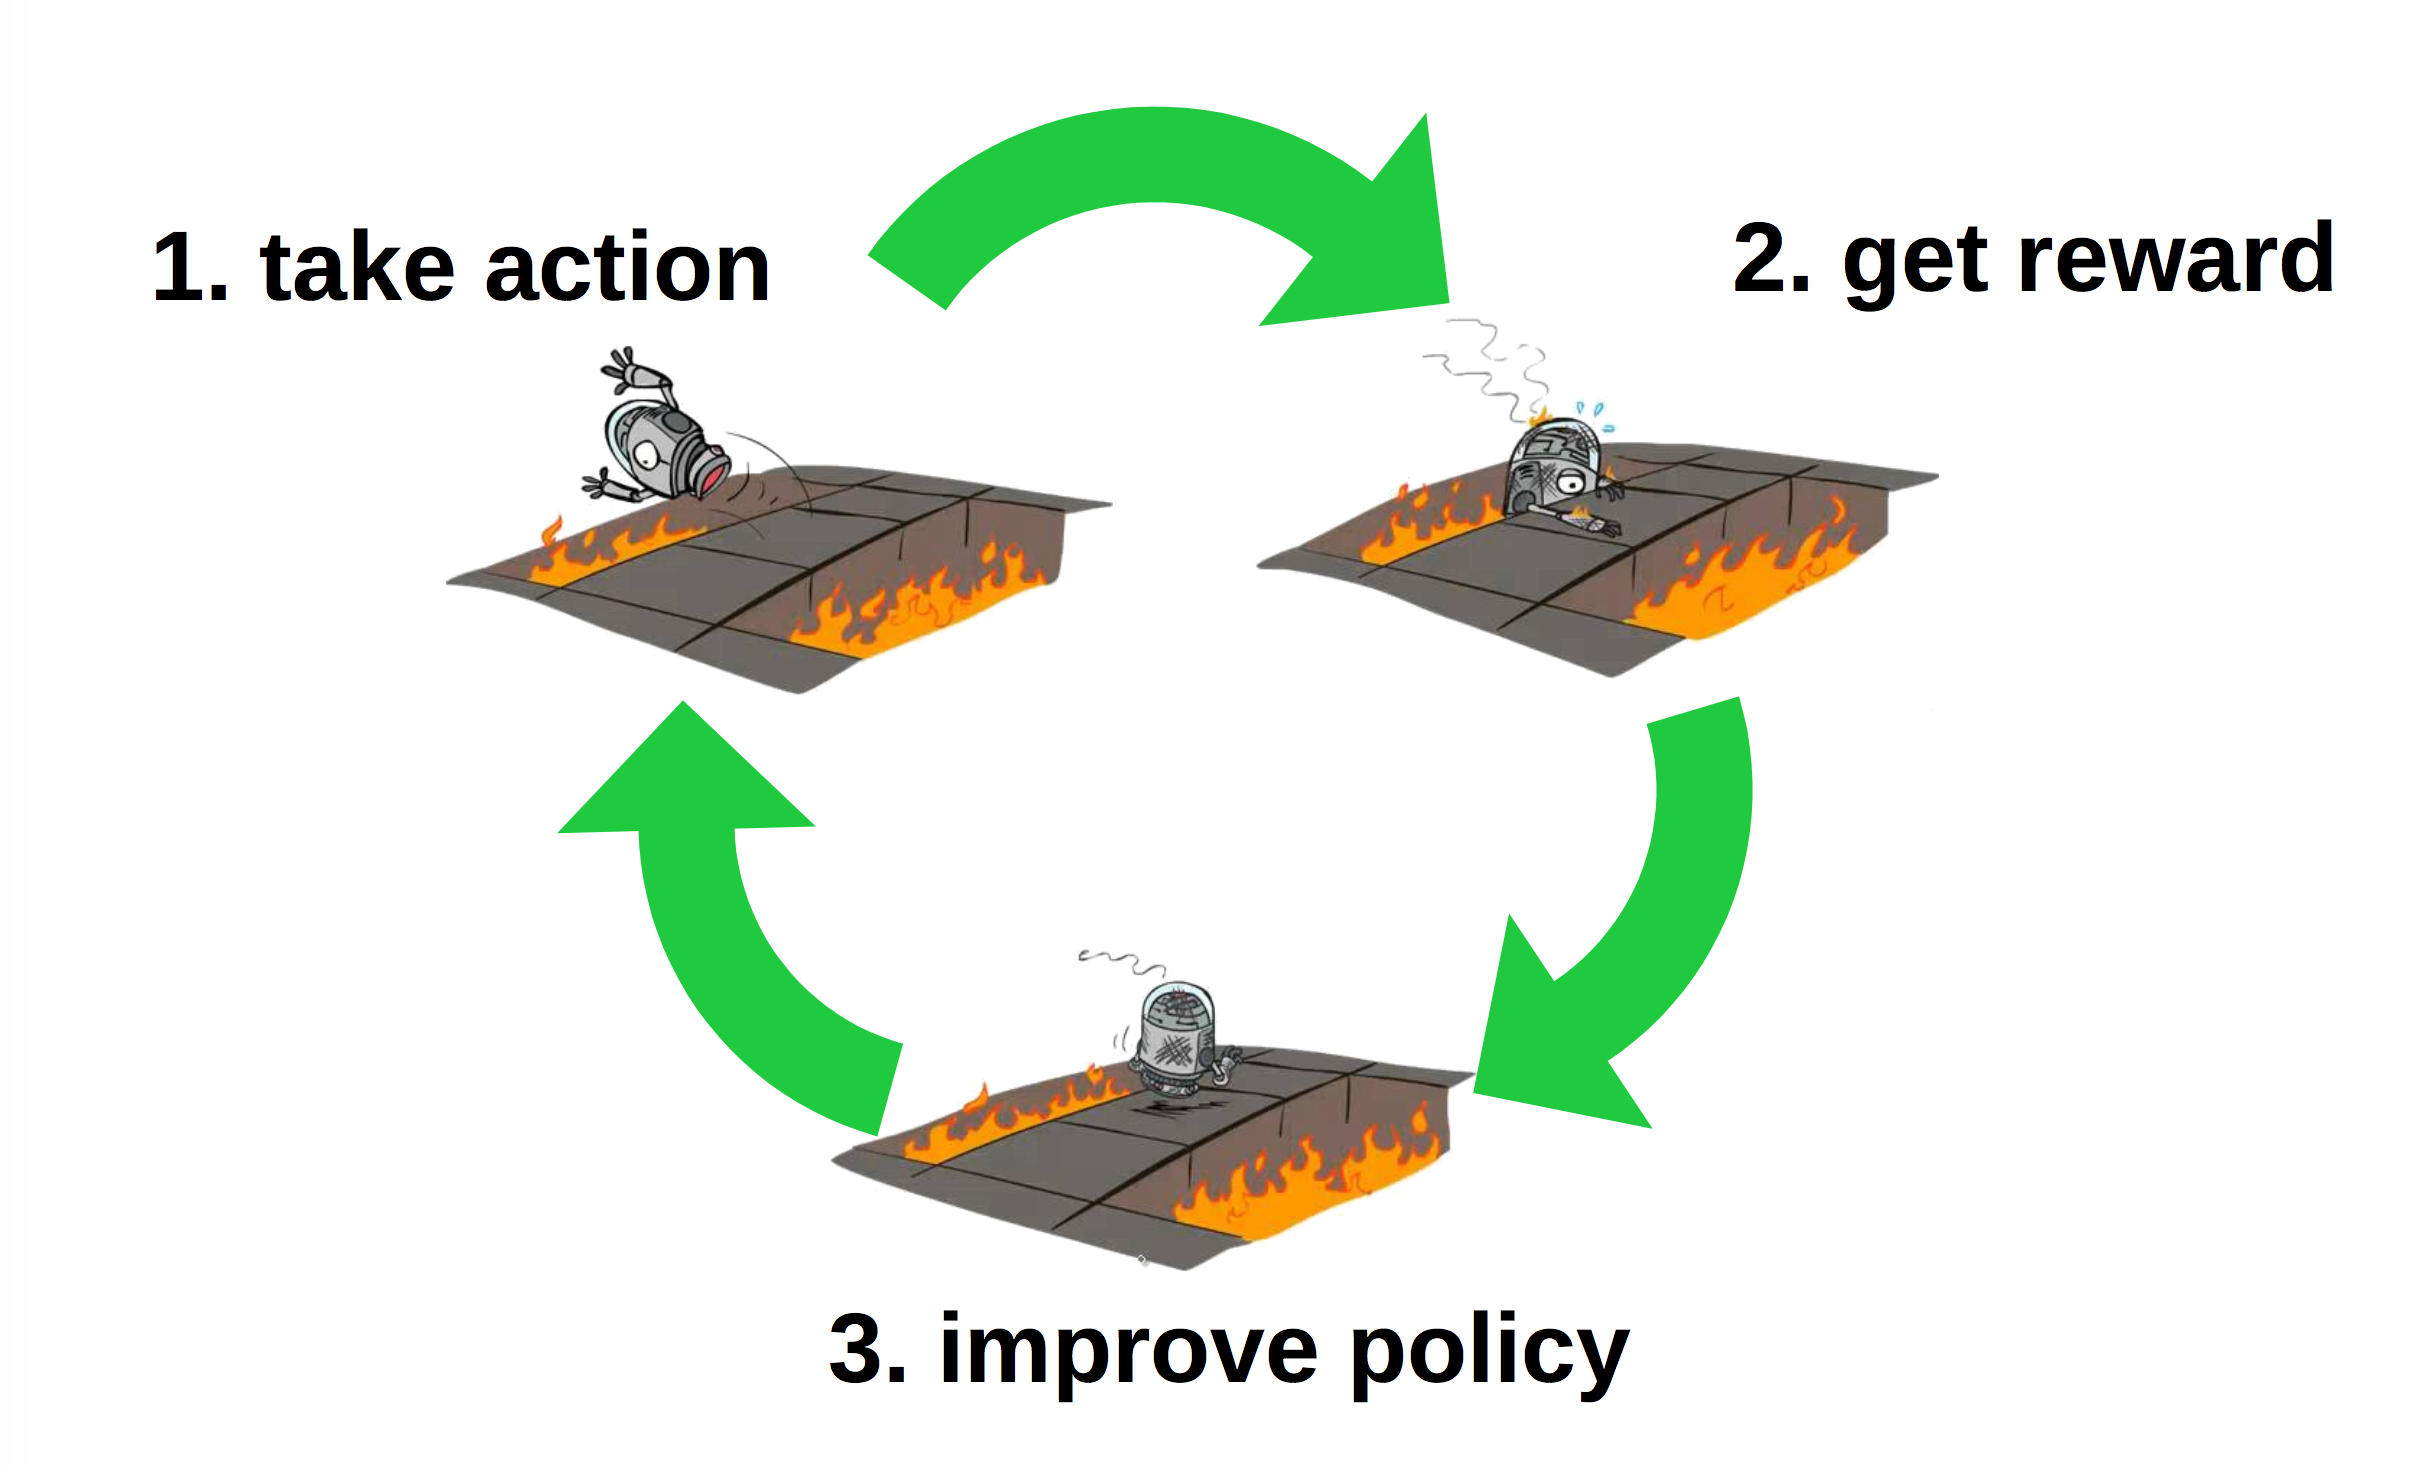
\includegraphics[width=.82\linewidth]{rl_easy1.png}
\end{center}
\end{frame}

\begin{frame}{Reinforcement Learning - это просто!}
\begin{center}
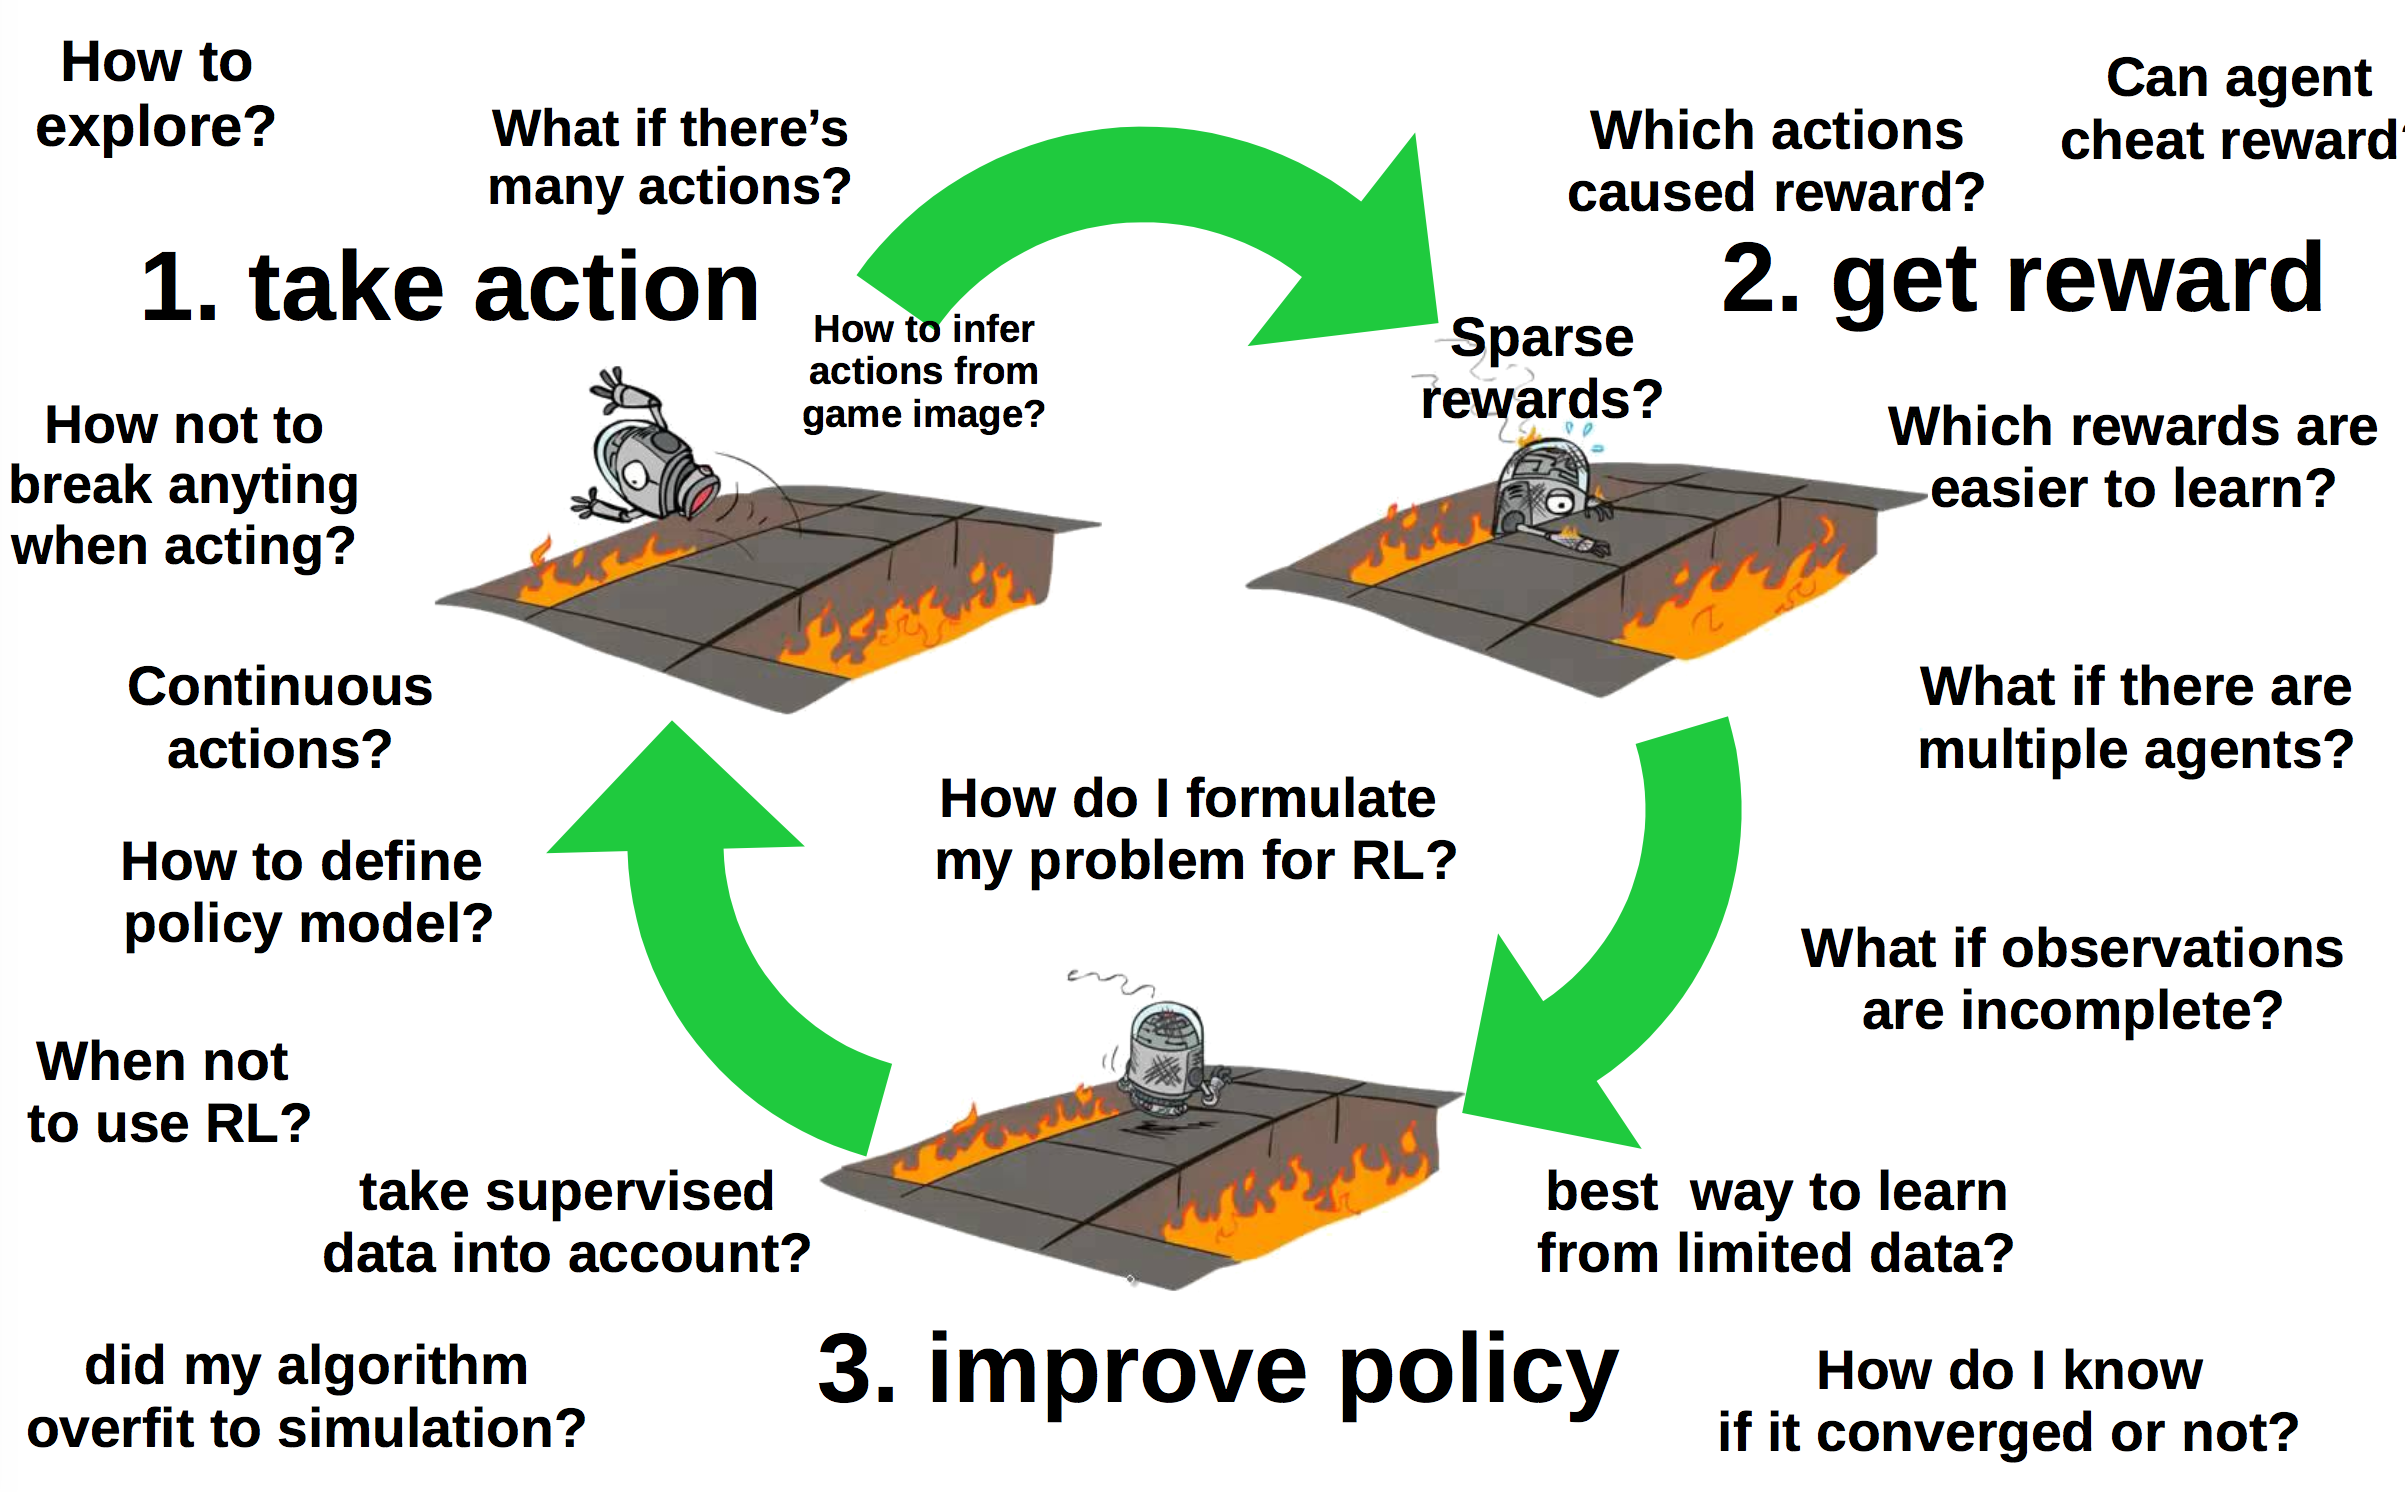
\includegraphics[width=.82\linewidth]{rl_easy2.png}
\end{center}
\end{frame}

%\begin{frame}{Deep Q Learning (DQN)}
%\begin{center}
%	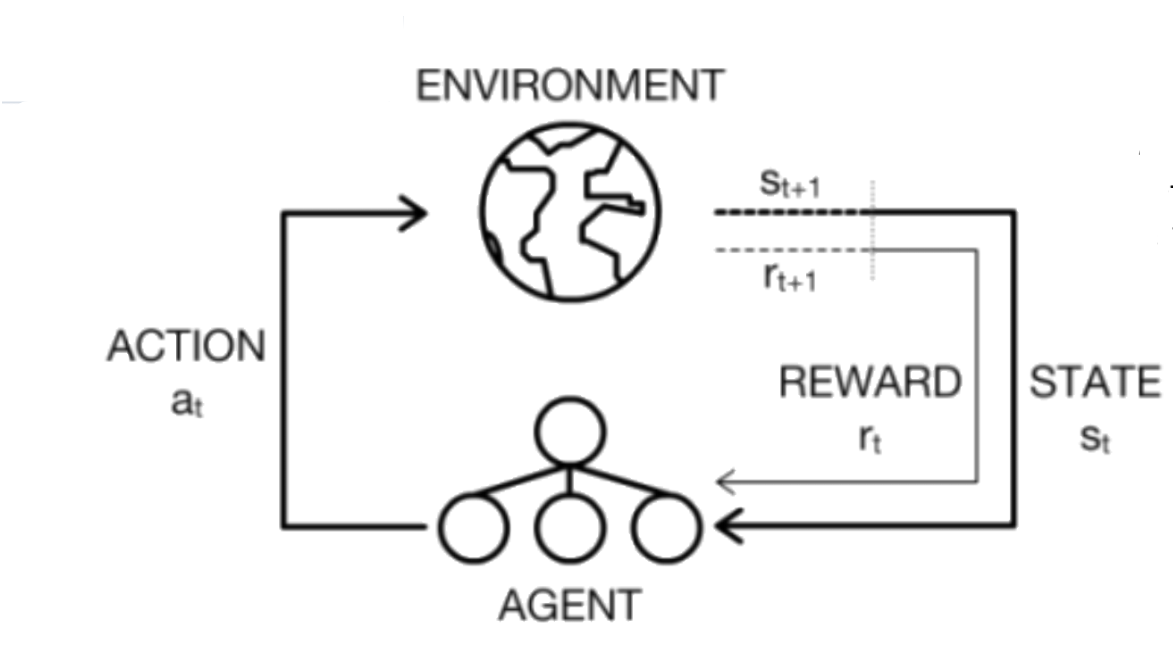
\includegraphics[width=.6\linewidth]{rl_1.png}
%\end{center}
%\begin{itemize}
%	\item  \alert{$Q(s,a)$ — Q-function,} сообщает ожидаемый reward для действия $a$ в состоянии $s$.
%\end{itemize}
%\end{frame}
%
%
%\begin{frame}{Deep Q Learning (DQN)}
%\begin{wideitemize}
%	\item  \alert{$Q(s,a)$ — Q-function,} сообщает ожидаемый  reward для действия $a$ в состоянии $s$.
%	
%	\item Пусть агент получил сейчас $r_t$, тогда в текущем периоде он хочет 
%	
%	\[ 
%	r_t + \gamma \cdot \max_{a} Q(s_{t+1}, a)
%	\]
%	
%	\item Изменение составит 
%	
%	\[
%	Q(s_{t+1}, a_{t+1}) =    r_t + \gamma \cdot \max_{a} Q(s_{t+1}, a) 
%	\]
%\end{wideitemize}
%\end{frame}
%
%
%\begin{frame}{Deep Q Learning (DQN)}
%
%\[
%Q(s_{t+1}, a_{t+1}) =    r_t + \gamma \cdot \max_{a} Q(s_{t+1}, a) 
%\]
%
%\begin{wideitemize}
%\item \alert{Оптимальная стратегия} —  что надо делать всю игру, чтобы получить максимальный выигрыш
%
%\item Если  у нас \alert{уже есть оптимальная функция $Q^{\ast}(s,a)$,} то играть мы можем следующим образом: в каждый момент времени $t$ спрашивать у этой функции как нам надо сходить, чтобы получить максимальный выигрыш. Ну а способ аппроксимировать сложные функции у нас уже есть —  нейронные сети!
%\end{wideitemize}
%\end{frame}
%
%
%\begin{frame}{Уравнение Белмана}
%
%
%\[
%Q(s_{t+1}, a_{t+1}) =    r_t + \gamma \cdot \max_{a} Q(s_{t+1}, a) 
%\]
%
%
%Следую нашей логике мы можем выписать уравнение Белмана:
%\begin{equation*}
%Q^{\ast}(s_t,a_t) = E _{s_{t+1}~\epsilon} [r+ \gamma max(Q^{\ast}(s_{t+1},a_{t+1}))|s_t,a_t]
%\end{equation*}
%
%Теперь мы хотим это все оптимизировать и приблизить. По сути получить следующую зависимость:
%\begin{equation*}
%Q(s,a;\Theta) \approx Q^{\ast}(s,a)
%\end{equation*}
%В данном случае у нас за $Q(s,a;\Theta)$ выступает нейронная сеть.
%\end{frame}
%
%
%
%\begin{frame}{Deep Q Learning (DQN)}
%
%\[
%Q(s_{t+1}, a_{t+1}) =   Q(s_t, a_t) + \alpha \cdot ( r_t + \gamma \cdot \max_{a} Q(s_{t+1}, a) - Q(s_t, a_t))
%\]
%
%\begin{wideitemize}
%	\item \alert{Оптимальная стратегия} - что надо делать всю игру, чтобы получить максимальный выигрыш
%	
%	
%	
%	
%	\item \alert{Динамическое программирование, уравнение Белмана}
%	
%	\item Это аналог поиска экстремума функции через производные, но уже в функциональном пространстве. Теория активно развивалась в 60-ые годы, как способ управлять ракетами, чтобы сбивать другие ракеты .
%\end{wideitemize}
%\end{frame}
%
%
%
%\begin{frame}{постановка задачи обучения с подкреплением}
% --  Вся эта 
%
%
%
%\end{frame}
%
%
%
%
%
%
%\begin{frame}{Обучение нейронной сети}
%Мы не можем напрямую брать производную по нашей функции. Но мы можем её итеративно приблежать (разворачивать во времени), шаг за шагом становится всё ближе. Сформулируем нашу ошибку для нейронной сети:
%\begin{gather*}
%L_i(\Theta_i) = E_{s,a} [(y_i - Q(s,a;\Theta_i)^2)]\\
%y_i = E _{s_{t+1}~\epsilon} [r+ \gamma max(Q^{\ast}(s_{t+1},a_{t+1};\Theta_i))|s_t,a_t]
%\end{gather*}
%
%\end{frame}
%
%%\begin{frame}{Алгоритм DQN}
%%\begin{center}
%%\includegraphics[width=.9\linewidth]{DQN.png}
%%\end{center}
%%\end{frame}
%%
%%\begin{frame}{Алгоритм DQN}
%%\begin{center}
%%\includegraphics[width=.4\linewidth]{SIMPLE_DQN.png}
%%\end{center}
%%\end{frame}
%
%\begin{frame}{Что получилось}
%\begin{enumerate}
%\item Хорошо играет в игры, где не нужна сильная и сложная стратегия (значительно лучше людей)
%\item Плохо играет в игры, где требуется смотреть на очень долгую перспективу (и если процесс не является марковским)
%\item Чем дальше итоговый выигрыш от каждого действия по времени, тем хуже модель справляется с обучением. Если я могу смотреть выигрыш каждый ход -- мир становится добрее.
%\end{enumerate}
%\end{frame}
%
%\begin{frame}{Сравнение}
%\begin{enumerate}
%\item Если работает -- работает стабильнее другого подхода к RL. Работает значительно реже.
%\item Существенно сложнее подхода policy gradients.
%\item Требует меньшего количества повторений (может использовать древние знания сети).
%\item Плохо исследует, требуется добавлять шум руками.
%\item Можно обучать на игре других, policy gradients нельзя.
%\end{enumerate}
%
%\end{frame}
%
%\begin{frame}{Играемся}
%Со всем этим делом можно поиграться в симуляторе (под питон) Gym. (\url{https://gym.openai.com/}).
%
%Относительно простой эмулятор части игр atari, который будет ждать наших шагов и получать от нас команды. Ставится через pip install и позволяет просто пытаться тренировать наши модели.
%
%\end{frame}
%


\end{document}




